% !TeX spellcheck = it_IT
\newpage
\section{Smart agricolture}
L'idea è di collegare dei sensori a dei bonsai che comunicano le misurazioni prima alla rete \textbf{fog} (locale) e poi eventualmente al cloud.
\begin{center}
	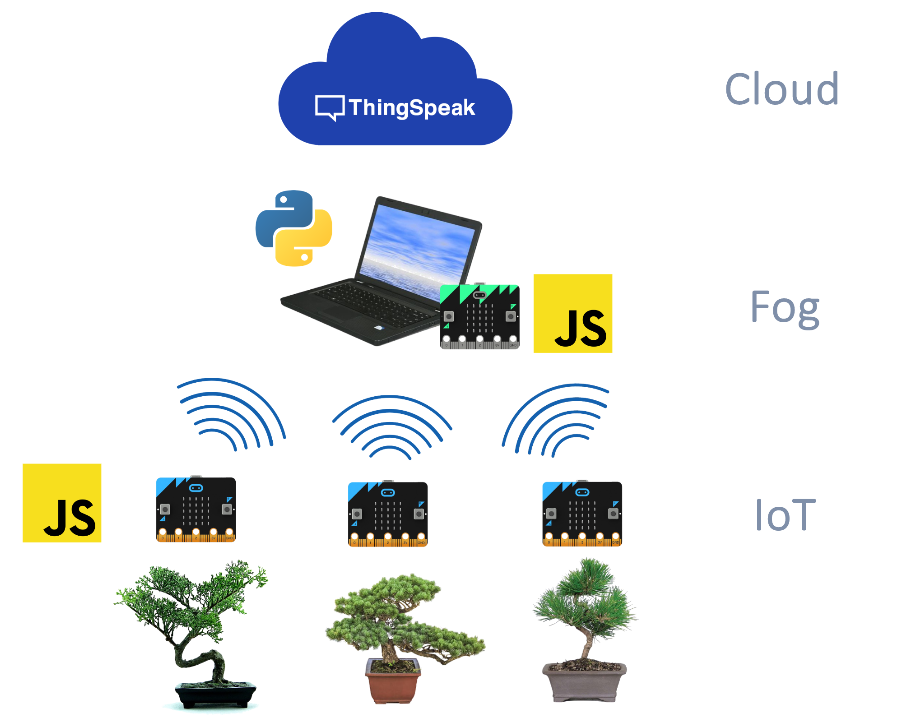
\includegraphics[scale=0.3]{bonsai_fog.png}
\end{center}
\subsection{IoT + Cloud}
\subsubsection{Sensori}
Il primo passo è quello di programmare i sensori per rilevare il livello di \textbf{umidità}:
\begin{lstlisting}[language=JavaScript]
	let reading = 0
	basic.forever(() => {
		reading = pins.analogReadPin(AnalogPin.P0)
		led.plotBarGraph(
			reading,
			1023
		)
		if (input.buttonIsPressed(Button.A)) {
			basic.showNumber(reading)
		}
	})
\end{lstlisting}
Dato che il sensore funziona a batteria, vogliamo ridurre i consumi. Per farlo, effettuiamo le misurazioni una volta al secondo invece che in continuazione.
\begin{lstlisting}[language=JavaScript]
	led.setBrightness(64)
	let reading = 0
	basic.forever(() => {
		pins.analogWritePin(AnalogPin.P1, 1023)
		reading = pins.analogReadPin(AnalogPin.P0)
		pins.analogWritePin(AnalogPin.P1, 0)
		led.plotBarGraph(
			reading,
			1023
		)
		if (input.buttonIsPressed(Button.A)) {
			basic.showNumber(reading)
		}
		basic.pause(1000)
	})
\end{lstlisting}
\newpage
Implementiamo ora la parte di comunicazione, mandando alla dashboard la misurazione e stampandola sul monitor seriale.
\begin{lstlisting}[language=JavaScript]
	radio.setTransmitSerialNumber(true)
	radio.setGroup(4)
	led.setBrightness(64)
	let reading = 0
	basic.forever(() => {
		pins.analogWritePin(AnalogPin.P1, 1023)
		reading = pins.analogReadPin(AnalogPin.P0)
		radio.sendNumber(reading / 4);
		pins.analogWritePin(AnalogPin.P1, 0)
		led.plotBarGraph(
			reading,
			1023
		)
		if (input.buttonIsPressed(Button.A)) {
			basic.showNumber(reading)
		}
		serial.writeValue("moisture", reading)
		basic.pause(1000)
	})
\end{lstlisting}
\subsubsection{Main}
In questo tipo di configurazione, tutti i dati verranno mandati direttamente al Cloud (\hyperref{https://thingspeak.com/}{}{}{ThingSpeak}).
\begin{center}
	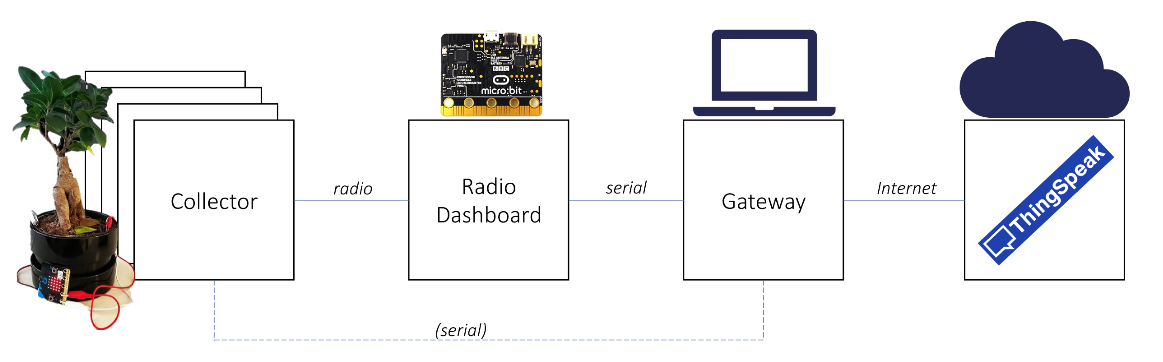
\includegraphics[scale=0.38]{bonsai_fog_cloud.png}
\end{center}
La capacità computazionale è enorme ma serve una connessione costante e introduciamo nel sistema un'alta latenza e un bottleneck di banda. Dobbiamo quindi filtrare le informazioni e processarle prima di inviarle, introducendo il livello \textbf{fog}. Ad esempio:
\begin{itemize}
	\item Aggregare i dati ed inviare una media ogni 10 secondi
	\item Inviare i dati solo se la differenza con la media precedente supera un certo valore
	\item Come al punto precedente, ma dopo un'ora inviare comunque il dato
\end{itemize}